\section{Introduction}
\label{sec:introduction}

An increasing number of swarm applications, both mobile and IoT applications,
are powered by machine learning (ML) to perform daily tasks. For example,
Microsoft SeeingAI~\cite{seeingai} is a talking camera for the blind and low
vision community that describes nearby people, text, objects. Wearable cognitive
assistant~\cite{ha2014towards} uses wearable devices, such as Google Glass, for
deep cognitive assistance (e.g., offering hints for social interaction via
real-time scene analysis).

Because of the close interaction with users, bounded response times is crucial
for a smooth experience. Previous studies~\cite{nielsen1994usability,
  schneiderman1998designing} have measured the effect of different end-to-end
latencies:

\begin{itemize}
\item 100 ms gives the feeling of instantaneous response.
\item 1 second keeps the user's flow of thought but users can sense the delay.
\item A few seconds' delay creates an unpleasant user experience.
\end{itemize}

While there is a staggering collection of research focusing on model
\textit{training}, these applications perform the \textit{inference} step of
machine learning: use trained models to make a prediction given an input, such
as visual~\cite{googlelens, ha2014towards, seeingai}, audio~\cite{alexa,
  applesiri, cortana}, and sensory information~\cite{laput2017synthetic,
  lu2010jigsaw}. Inference has received relatively little attention, especially
on end and edge devices.

%% Reference:
%% https://www.nngroup.com/articles/website-response-times/

%% 0.1 seconds gives the feeling of instantaneous response — that is, the
%% outcome feels like it was caused by the user, not the computer. This level of
%% responsiveness is essential to support the feeling of direct manipulation
%% (direct manipulation is one of the key GUI techniques to increase user
%% engagement and control — for more about it, see our User Interface Principles
%% Every Designer Must Know course).

%% 1 second keeps the user's flow of thought seamless. Users can sense a delay,
%% and thus know the computer is generating the outcome, but they still feel in
%% control of the overall experience and that they're moving freely rather than
%% waiting on the computer. This degree of responsiveness is needed for good
%% navigation.

%% 10 seconds keeps the user's attention. From 1–10 seconds, users definitely
%% feel at the mercy of the computer and wish it was faster, but they can handle
%% it.

%% There are also some great discussion about latency here:
%% https://danluu.com/term-latency/

\begin{figure}
  \centering
  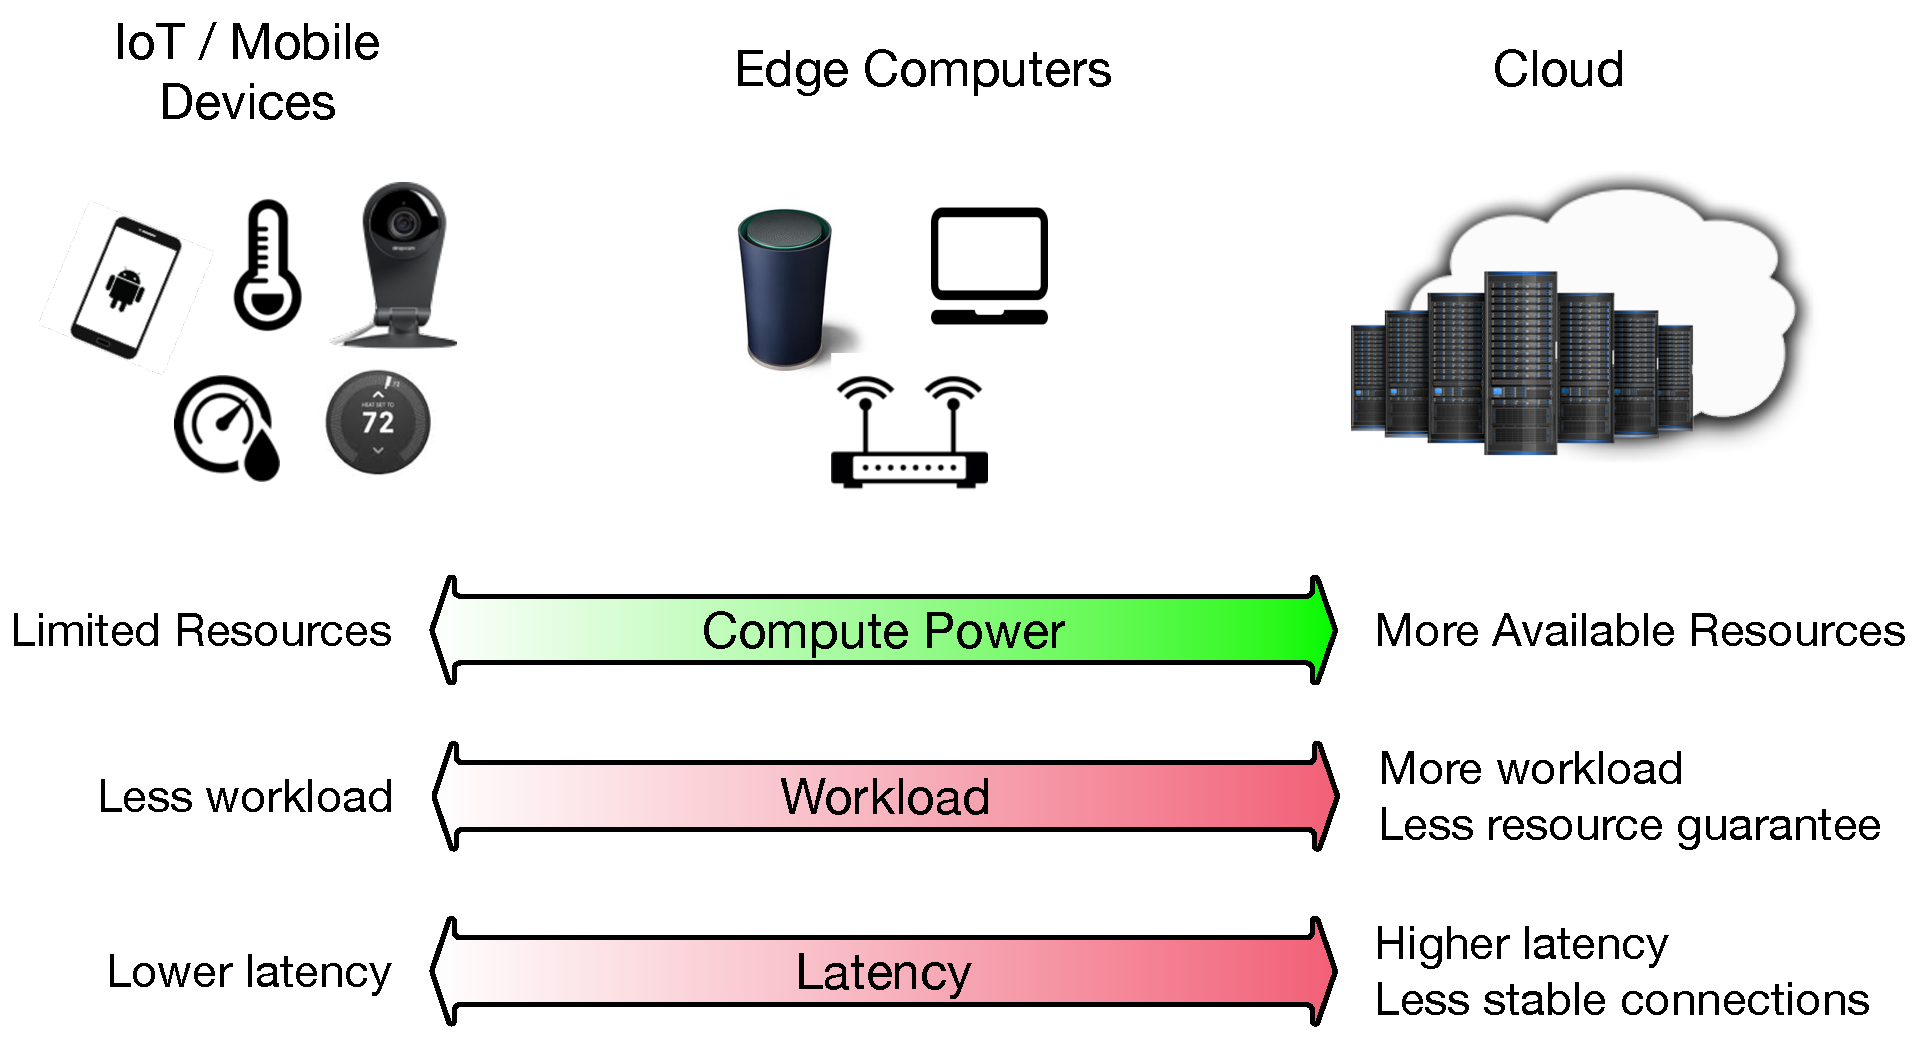
\includegraphics[width=0.8\columnwidth]{figures/background.pdf}
  \caption{Characteristics of IoT/mobile, edge and cloud.}
  \label{fig:mobile-edge-cloud}
\end{figure}

We illustrate the spectrum of resources, workload and latency among end devices,
the edge and the cloud in \autoref{fig:mobile-edge-cloud}.

Performing inference on swarm platforms with bounded response times has remained
challenging, especially for heavy computations beyond the capabilities of end
devices. State-of-the-art computer vision algorithms, such as object detection,
easily take several seconds on modern smartphones~\cite{chen2015glimpse}.

Prior work explores offloading~\cite{chun2011clonecloud,cuervo2010maui} to the
cloud or the edge\footnote{Also referred to as
  cloudlet~\cite{satyanarayanan2009case}, the fog~\cite{bonomi2012fog}.}  that
hosts machine learning models and performs heavy computation. Despite their
powerful computing capability and more available resources---including special
hardware like GPU and TPU~\cite{jouppi2017datacenter}---these platforms suffer
from increased network latency and service overload, thus unable to meet latency
goals consistently.

Redundant requests is one technique to address the variability in network
delays~\cite{gordon2015accelerating, vulimiri2013low} and slow servers (known as
straggler mitigation in the cloud~\cite{dean2013tail,
  ananthanarayanan2013effective}). These systems initiate multiple requests
across diverse resources and use the first result which completes. While
effective, existing work treats these resources equally and executes the same
task on them. This is a poor match for the heterogeneous swarm space.

Our insight is that for a particular inference task, multiple algorithms or
tunable parameters for one algorithm exist that requires different processing
times and result in different accuracy. To accommodate the resource-constrained
devices, one can use an algorithm or a parameter that suits the particular
platform.

\begin{figure}
  \centering
  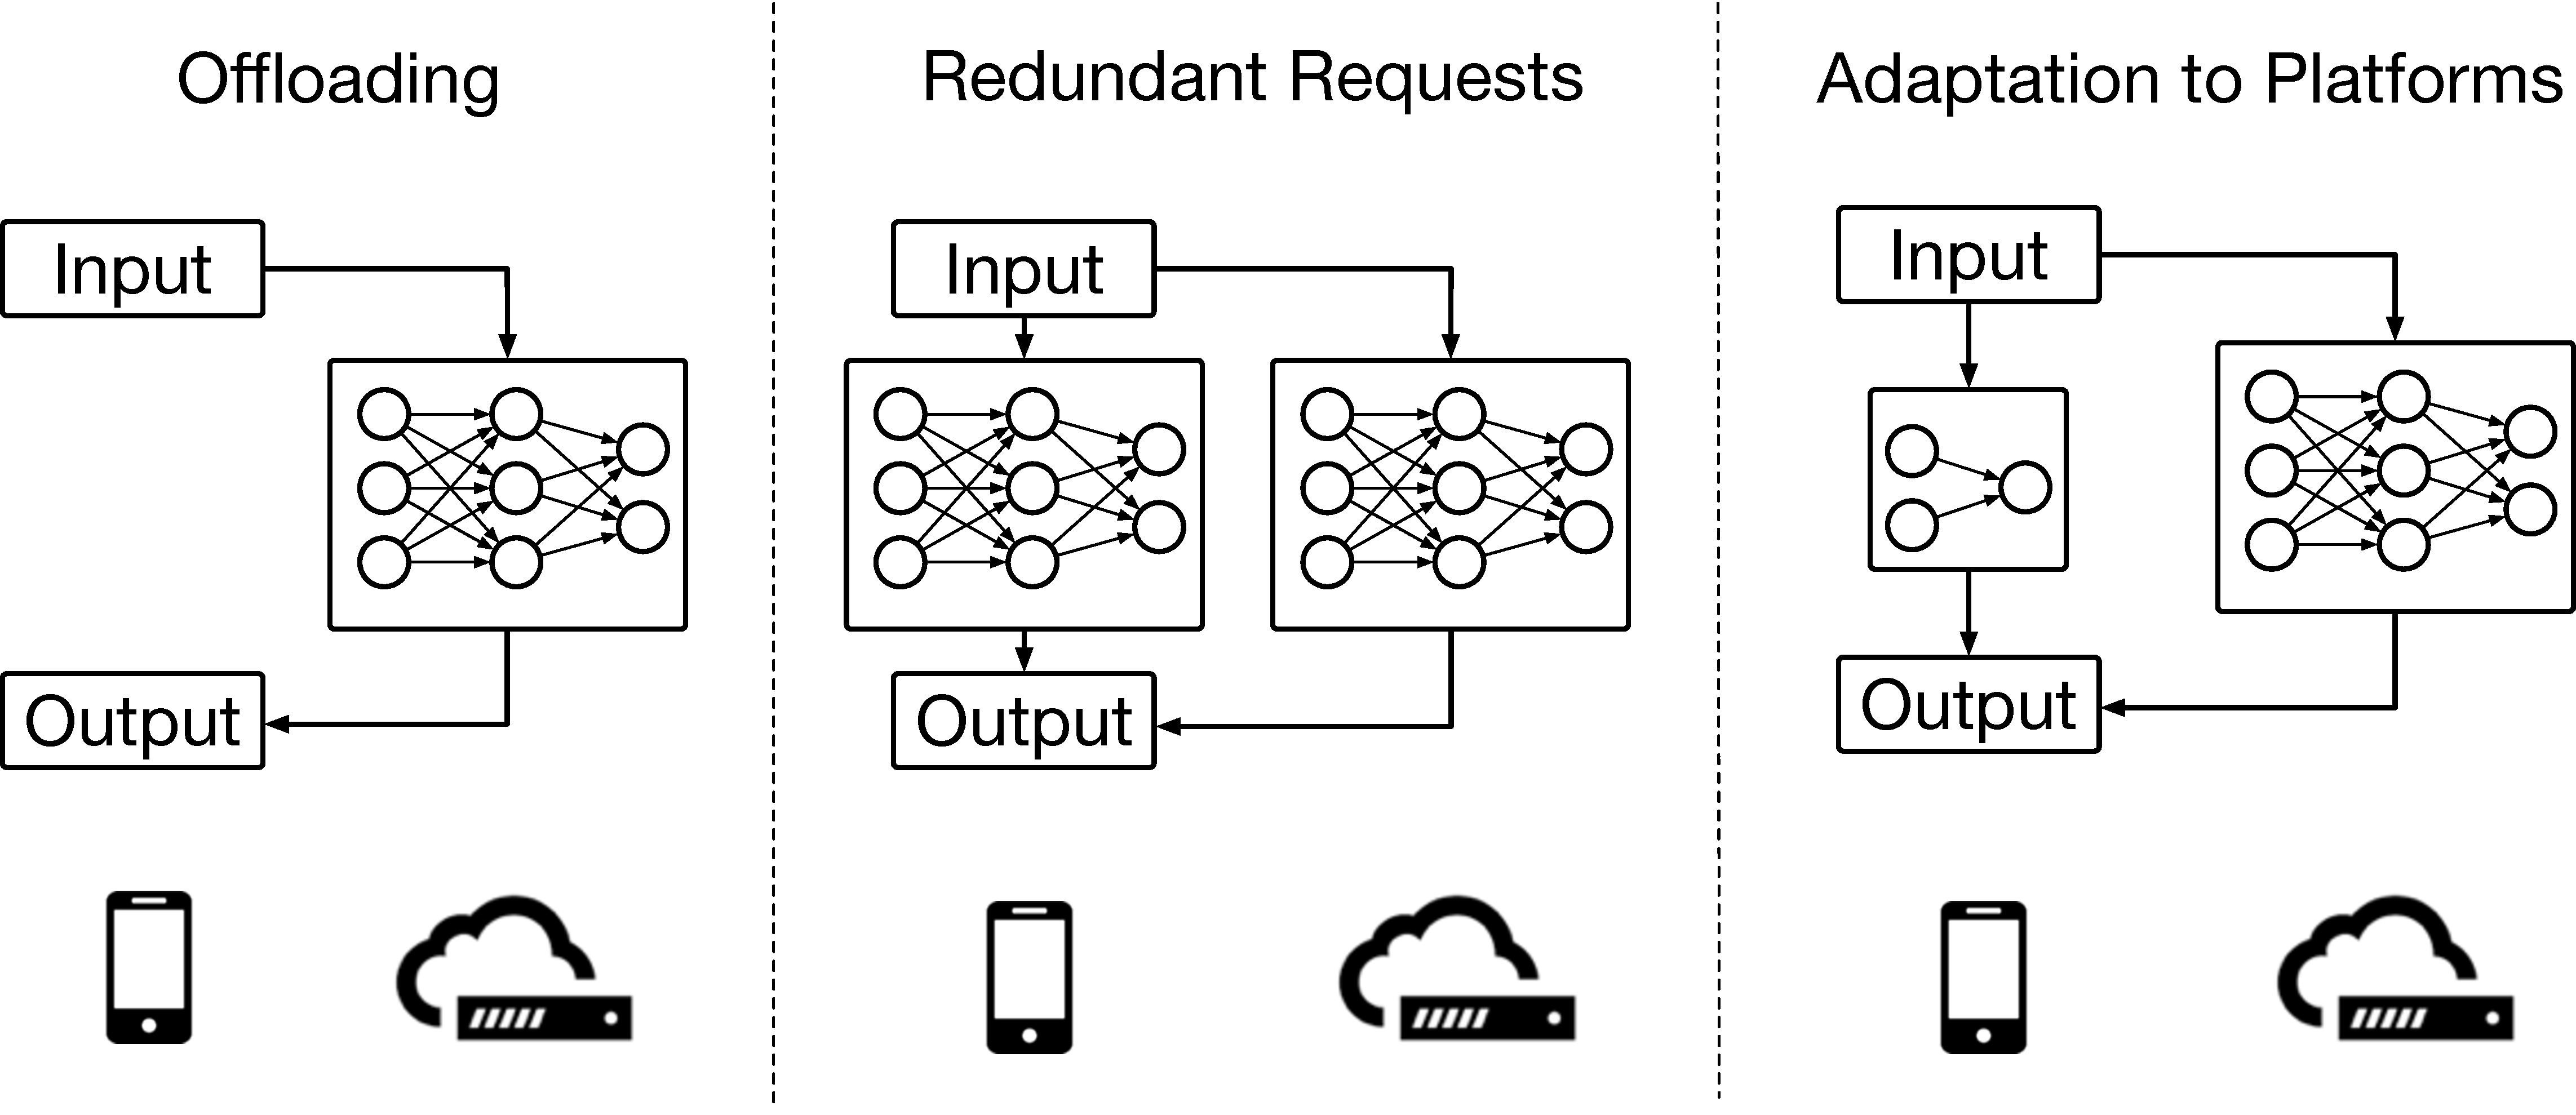
\includegraphics[width=0.8\columnwidth]{figures/dr.pdf}
  \caption{Illustration of offloading, redundant requests and differential
    redundancy.}
  \label{fig:dr}
\end{figure}

We propose to adapt the computation (as in \autoref{fig:dr}) to each individual
platform by leveraging the choices of algorithms and parameters for a particular
inference task. With a precise performance model that captures the tradeoff
space between application accuracy and processing times, we can achieve such
adaptation and then bounded response times. This adaptation technique is
orthogonal to existing system solutions, such as scale-out, scale-up, caching,
or batching.

On the client side, it uses the configuration best suited for its particular
hardware capability.

On the server side, each request is annotated with a service-level objective
(SLO) that describes the deadline and accuracy demand. Upon receiving a request,
the server runs a real-time scheduler to meet all SLOs. $(i)$ \brt{} can adjust
each request's serving time and quality based on the profile; $(ii)$ \brt{} is
allowed to reject a request because of the redundancy mentioned above.

Because \brt{} is application-aware, it requires knowledge from the application
developer. And therefore a well-designed abstraction.

Efficient profiling to find the performance model. In order to explore the
trade-off space, we take a data-driven approach to learn the relationship
between inference accuracy and processing times for each algorithm and different
parameters for individual platforms. We call this process ``profiling'' and its
goal is to find Pareto-optimal configurations (algorithm and parameter) as the
performance model.

Profiling with an exhaustive search may not be feasible for some algorithms due
to their large parameter space. In these cases, we use a statistical method,
Bayesian Optimization (BO), to model the relationship as a black-box function
and only searches for near-optimal configurations.

Profiling for all hardware platforms is not feasible due to the large space and
availability of the hardware at development time. We observe that the profile
can be easily transferred across platforms with linear transformation.

We make the following contributions in this chapter with \brt{}:

\begin{itemize}

\item The proposed Bayesian Optimization (BO) for profiling, significantly
  outperforms previous approaches with random search or coordinate/greedy
  approach.
\item We empirically validate the profile transfer to address heterogeneous
  capabilities across swarm platforms.

\end{itemize}

% \begin{figure*}
%   \centering
%   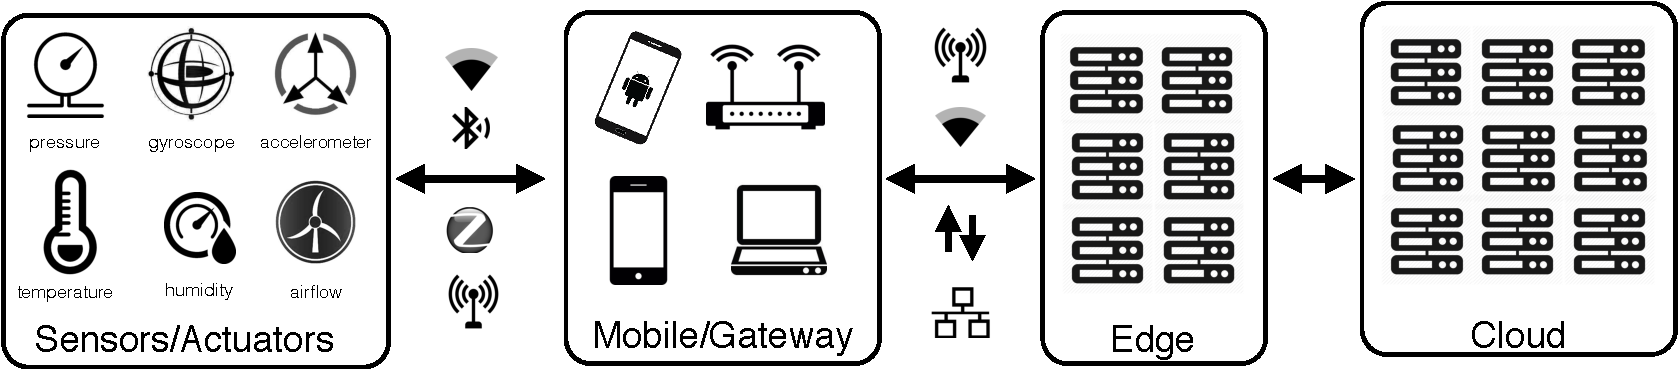
\includegraphics[width=\textwidth]{figures/platforms}
%   \label{fig:options}
%   \caption{Platforms}
% \end{figure*}

%%% Local Variables:
%%% mode: latex
%%% TeX-master: "../compute"
%%% End:
